\documentclass[11pt]{article}
\usepackage[utf8]{inputenc}
\usepackage[T1]{fontenc}
\usepackage[spanish]{babel}
\usepackage{amsmath}
\usepackage{amsfonts}
\usepackage{amssymb}
\usepackage{graphicx}
\usepackage{caption}
\usepackage{wrapfig}
\usepackage{subcaption}
\usepackage{textcomp}
\usepackage{siunitx}
\usepackage{geometry}
\usepackage{courier}
\usepackage{cancel}
\spanishdecimal{.}

\title{Física Numérica}
\author{Julio César Avila Torreblanca}
\date{14 de octubre del 2021}

\setlength{\parindent}{0cm}
\geometry{verbose,tmargin=1in,bmargin=1in,lmargin=1in,rmargin=1in}
\begin{document}
\maketitle

\section*{Tarea 5}
\subsection*{\textbf{1. Estudiando la evolución de la temperatura en una barra}}
\begin{enumerate}
	\item [\textbf{(a)}] Considere una barra cilíndrica de aluminio de longitud $L= 1$ m y un grosor $\omega$ colocada a lo largo del eje $x$. Dicha barra se encuentra aislada termicamente a lo largo de su longitud, pero no en sus extremos. Inicialmente la barra se encuentra a una temperatura uniforme de $T_0 = 100$ °C, y los extremos se encuentran en contacto con una barra de hielo a 0 °C. El calor fluye a través de los extremos no aislados. ¿Cuál es la ecuación que modela este proceso?, ¿Qué tipo de ecuación es?, ¿Puede resolverla analíticamente?, ¿Qué métodos de solución conoce para este tipo de ecuaciones?, ¿Hay condiciones de frontera asociadas?.
\end{enumerate}
\textit{Solución.}\\
	 La ecuación que relaciona el flujo del calor con el gradiente de temperatura $T$ a través del material, es la llamada \textit{Ecuación de calor}:
	 \begin{equation}
	 	\frac{\partial T (\vec{x},t)}{\partial t} = \frac{K}{C \rho} \nabla^2 T (\vec{x},t)		\label{1}
	 \end{equation} 
	 
	 Donde $K$ es la conductividad térmica del material, $C$ el calor específico y $\rho$ su densidad. Además la temperatura $T$ es función del tiempo $t$ y del vector espacial $\vec{x}$. La ecuación de calor (1) es una ecuación diferencial parcial parabólica, cuyas variables independientes son temporales y espaciales.  
	 Notemos que la temperatura en la barra cilíndrica es uniforme, y el flujo de calor también lo es. Debido a esta simetría, es posible considerar nuestro problema en una sola dimensión, es decir, considerar la barra cilíndrica como un alambre en el eje $x$ cuyos extremos se encuentran en $x=0$ y $x=L$. De esta forma, la ecuación que describe el problema se reduce a:
	 \begin{equation}
	 	\frac{\partial T (x,t)}{\partial t} = \kappa \frac{\partial^2 T (x,t)}{\partial x^2}	\label{2}
	 \end{equation}
	 
	 Donde hemos definido la constante:
	 
	 $$\kappa = \frac{K}{C \rho}$$
	 
	 Notemos que la ecuación (2) es fácil de resolver analíticamente si se utiliza separación de variables. Es decir, proponer una solución de la forma:
	 
	 $$T(x,t) = X(x)F(t)$$
	 
	 Por otra parte, la barra inicialmente tiente una temperatura uniforme  $T_0 =100$ °C. Por lo que nuestra primer condición de frontera es:
	 
	 $$T(x ,0) = 100 \text{C}$$
	 
	 Por otro lado, en  cualquier instante de tiempo posterior, los extremos de la barra que están en contacto con el hielo permanecerán a 0 ° C. Así nuestra segunda y tercer condición de frontera resultan:
	 
	 $$T(0 ,t) = T (L,t) = 0 °\text{C}$$

\begin{enumerate}
	\item [\textbf{(b)}] ¿Cómo podría resolver numéricamente el problema?¿Tiene algún algoritmo que podría ayudarle?
\end{enumerate}
\textit{Solución.}\\
	Para poder resolver la ecuación (2) de forma numérica se requiere de un algoritmo que permita calcular derivabas numéricamente. Nos apoyaremos del algoritmo de *Foward difference* y *Central difference* para calcular las derivadas parciales.  
	Para la derivada respecto del tiempo, debido a que el fenómeno sucede para $t\geq 0$ usaremos aproximación por *Foward difference*. Es decir:
	
	$$\frac{\partial T(x,t)}{\partial t} \approx \frac{T(x, t + \Delta t) - T(x,t)}{\Delta t}$$
	
	Por otro lado, para la derivada espacial tenemos mayor libertad ya que se conoce la temperatura a lo largo de todo el segmento. Aquí podemos usar *Central difference*. Aplicando este algoritmo dos veces, obtenemos la aproximación para la segunda derivada:
	
	$$\frac{\partial^2 T(x,t)}{\partial x^2} \approx \frac{T(x +\Delta x , t) + T(x - \Delta x,t) - 2T(x,t)}{(\Delta x)^2}$$
	
	Sustituyendo estas aproximaciones en (2):
	
	$$ \frac{T(x, t + \Delta t) - T(x,t)}{\Delta t} = \kappa  \frac{T(x +\Delta x , t) + T(x - \Delta x,t) - 2T(x,t)}{(\Delta x)^2}$$
	
	Reescribiendo:
	
	\begin{equation}
		T(x, t + \Delta t) = T(x,t) + \frac{\kappa\Delta t}{(\Delta x)^2} \left[ T(x + \Delta x , t) + T(x - \Delta x,t) - 2T(x,t) \right] \label{3}
	\end{equation}
	
	Si definimos: 
	
	$$\eta = \frac{\kappa\Delta t}{(\Delta x)^2} = \frac{K \Delta t}{C\rho (\Delta x)^2}$$
	
	Y discretizando a $x$, $t$ de la forma:
	
	$$x = i \Delta x\quad;\quad t=j\Delta j$$
	
	Además:
	
	$$T(x,t)= T(i\Delta x , j \Delta t) = T_{ij}$$
	
	Nuestra ecuación (3) se reescribe como:
	
	\begin{equation}
		T_{ij+1} = T_{ij} + \eta \left[ T_{i+1 j } + T_{i-1 j} - 2T_{ij} \right]	\label{4}
	\end{equation}

	Esta relación de recurrencia permite conocer la temperatura en un instante de tiempo posterior $j+1$ para un punto espacial fijo $i$, a partir de conocer la temperatura en los puntos espaciales vecinos $i\pm1 $ en el instante de tiempo $j$ y la temperatura para ese punto $i$ en ese mismo timepo $j$. Debido a la condición de frontera:
	
	$$T(x ,0) = 100 \text{°C},\quad \forall x$$
	
	Es posible determinar la temperatura en cualquier instante de tiempo.  
	Para generar un algoritmo que permita resolver esta ecuación diferencial de forma numérica, utilizaremos el programa visto en clase. El código es el siguiente:
	\begin{figure}[h]
		\centering
		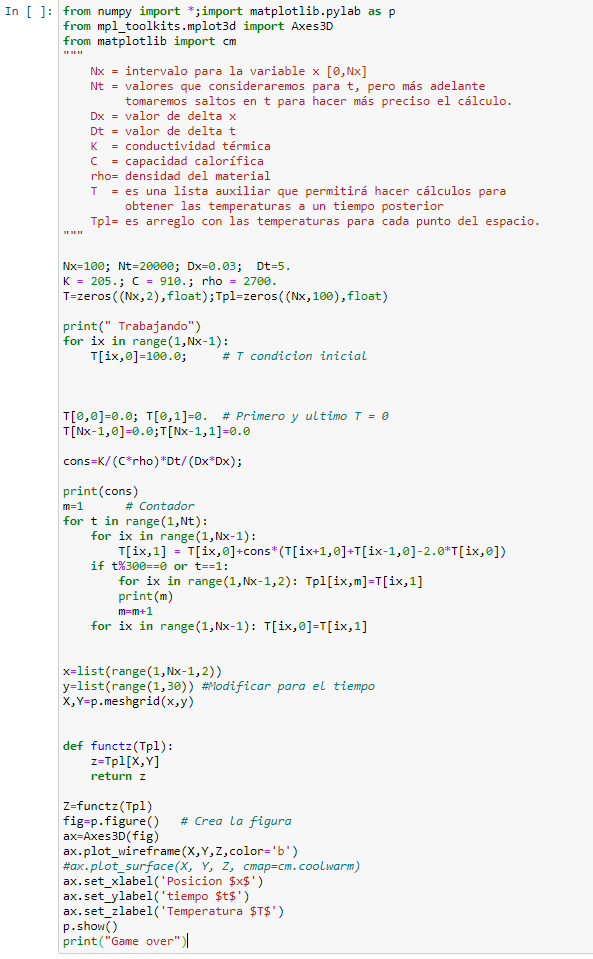
\includegraphics[width=10.5cm]{Img/Calor.PNG}
		\caption{Algoritmo para resolver numéricamente la ecuación de Calor.}
		\label{A1}
	\end{figure}
	
	Donde se ha definido a $\Delta x = 0.03$ y $\Delta t = 5.0|$. Además, se han usado los siguientes valores para el aluminio:
	\begin{equation}
		K = 205\,\, \si{W/(m\cdot K)},\quad C= 910\,\, \si{J/(kg\,\, K)},\quad \rho = 2700 \,\,\si{kg/m^3}	\label{valoresal}
	\end{equation}
\begin{enumerate}
	\item [\textbf{(c)}] Ya que tenga un programa que le ayude a resolver numéricamente	el problema, varíe los pasos en el tiempo y en el espacio en sus cálculos para obtener soluciones que sean estables y varíen suavemente tanto en tiempo como en espacio.
\end{enumerate}
\textit{Solución.}\\	
	En el algoritmo usado se tuvo que variar las variables \texttt{Nx}, \texttt{Nt}, \texttt{Dx} y \texttt{Dt}, además de ajustar el tamaño de los arreglos \texttt{Tpl} y \texttt{y} de acuerdo a los valores ingresados. Los valores encontrados para generar una solución estable y suave en todo el espacio fueron los siguientes:
	\begin{align}
		\texttt{Nx} = 100,\quad \texttt{Nt} = 20000, \quad \texttt{Dx} = 0.03, \quad \texttt{Dt} = 5.0 \label{valores1}
	\end{align}
	En la figura (\ref{A1}) se aprecia la asignación de estos valores al inicio del código. Con esto, se logró obtener un gráfico 3D para analizar el cambio de temperatura a lo largo de toda la barra en distintos instantes de tiempo. El gráfico generado fue el siguiente:
	
	\begin{figure}[h]
		\centering
		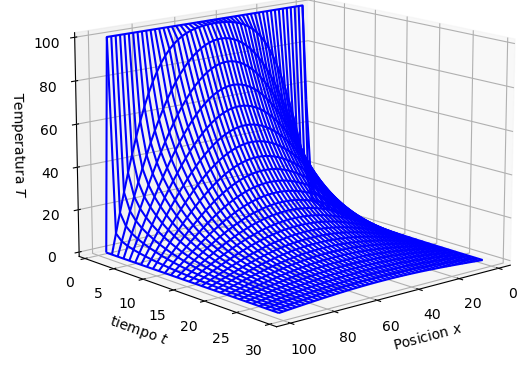
\includegraphics[width=10cm]{Img/G1.png}
		\caption{Temperatura en lo largo de  barra de Aluminio a distintos tiempos.}
		\label{G1}
	\end{figure}

	Se puede apreciar que en $t=0$ la temperatura a lo lardo de la barra era $T = 100 \text{°C}$. Después de ello, fue disminuyendo suavemente hasta que alcanzar el equilibrio térmico en toda la barra.
	
\begin{enumerate}
	\item [\textbf{(d)}] Pruebe qué pasa cuando la condición de estabilidad de Neumann/Courant
	no se satisface.
\end{enumerate}
\textit{Solución.}\\
	La condición de Neumann/Courant para este problema es la siguiente:
	\begin{equation}
		\eta = \frac{K \Delta t }{C\rho (\Delta x)^2}<\frac{1}{2} \label{condicion}
	\end{equation}
	Sustituyendo los valores considerados en (\ref{valoresal}) y(\ref{valores1}), tenemos que el valor considerado en el inciso (c) fue:
	$$\eta =\frac{(205)(5.0)}{(910)(2700)(0.03)^2}\approx 0.46<\frac{1}{2}$$
	Como se cumplió la condición de Neumann/Courant, la solución obtenida fue estable. Veamos que valor asignar a $\frac{\Delta t}{(\Delta x)^2}$ para no cumplir esta condición. Despejando de (\ref{condicion}) encontramos que:
	\begin{equation}
		\frac{\Delta t}{(\Delta x)^2} < \frac{C\rho}{2 K } \approx 5993	\label{cond}
	\end{equation}
	Así:
	$$\Delta t < 5993 (\Delta x)^2$$
	Si tomamos a $\Delta x = 0.03$ entonces: 
	$$\Delta t < 5.39$$
	Así que, esta es la condición que debe cumplir $\Delta t$ para tener estabilidad en la solución. A continuación presentamos varios gráficos donde se vario el valor de $\Delta t$ para observar el comportamiento de nuestra solución:
	\begin{figure}[h]
		\begin{subfigure}[b]{0.49\textwidth}
			\centering
			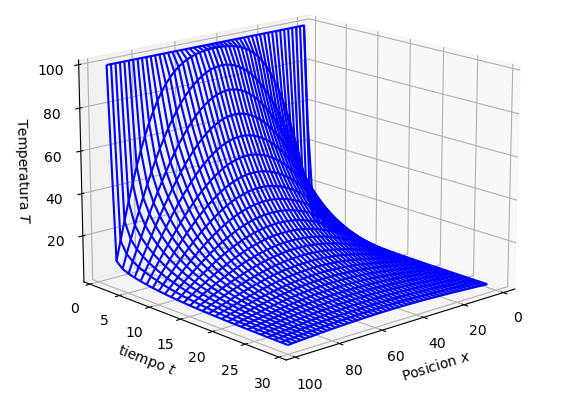
\includegraphics[width=8cm]{Img/5.3.png}
			\caption{Gráfico con $\Delta t = 5.30$}
			\label{}
		\end{subfigure}
		\hfill
		\begin{subfigure}[b]{0.49\textwidth}
			\centering
			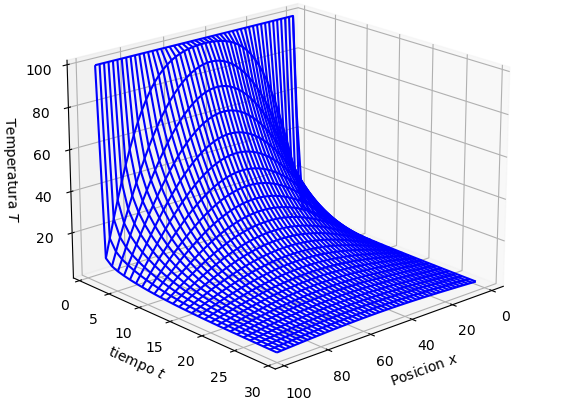
\includegraphics[width=8cm]{Img/5.39.png}
			\caption{Gráfico con $\Delta t = 5.39$}
			\label{}
		\end{subfigure}
		\caption{}
	\end{figure}

	\begin{figure}[h]
		\begin{subfigure}[b]{0.49\textwidth}
			\centering
			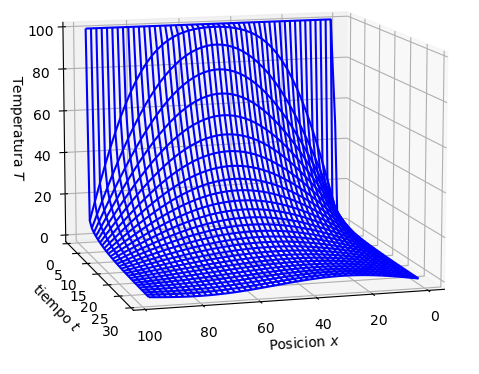
\includegraphics[width=8cm]{Img/5.4.png}
			\caption{Gráfico con $\Delta t = 5.40$}
			\label{}
		\end{subfigure}
		\hfill
		\begin{subfigure}[b]{0.49\textwidth}
			\centering
			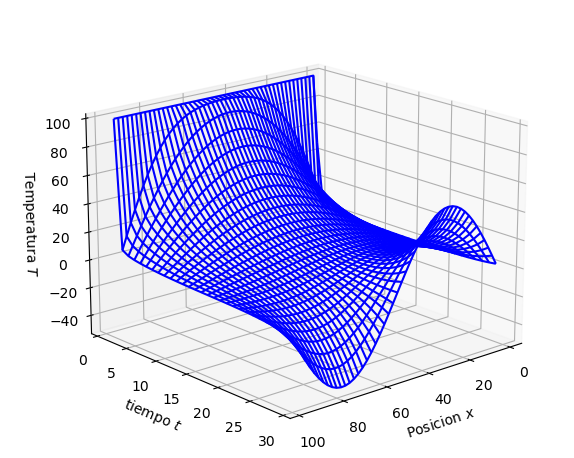
\includegraphics[width=8cm]{Img/5.401.png}
			\caption{Gráfico con $\Delta t = 5.401$}
			\label{}
		\end{subfigure}
		\caption{}
	\end{figure}
\newpage
	\begin{figure}[h]
		\centering
		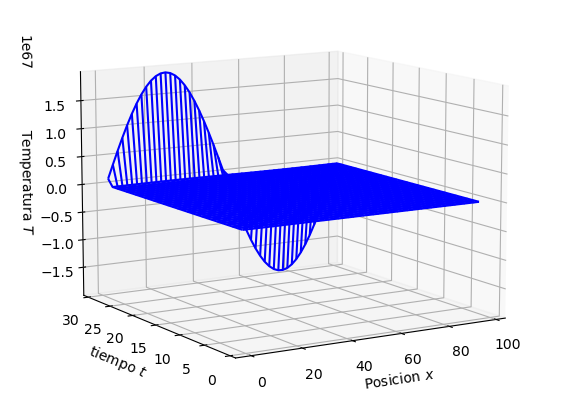
\includegraphics[width=8cm]{Img/5.45.png}
		\caption{Gráfico con $\Delta t = 5.45$}
		\label{}
	\end{figure}

	Podemos ver que que para $\Delta t = 5.30$ y $\Delta t =5.39$ la solución sigue comportándose suavemente. Pero en $\Delta t = 5.40$ se comienza a ver una pequeña perturbación en $t=30$ que no es de esperarse. Luego en $\Delta t = 5.401$, se aprecia mucho mejor que ya nuestra solución no es estable, pues la gráfica se comporta de forma anormal. Por último, cuando $\Delta t = 5.45$ la solución es completamente inestable. La gráfica resultante no dice nada respecto al problema, esto debido a que en los cálculos hechos por la computadora se acerca al overflow y comienza a tener errores con la interpretación de los resultados. 
	
	
\begin{enumerate}
	\item [\textbf{(e)}]  Revise que sus resultados concuerden con las condiciones de frontera establecidas.
\end{enumerate}
\textit{Solución.}\\	
	Nuevamente analicemos la solución dada en el inciso (c) vista desde otro ángulo, donde hemos tomado los valores (\ref{valoresal}) y (\ref{valores1}):
	\begin{figure}[htp!]
		\begin{subfigure}[b]{0.48\textwidth}
			\centering
			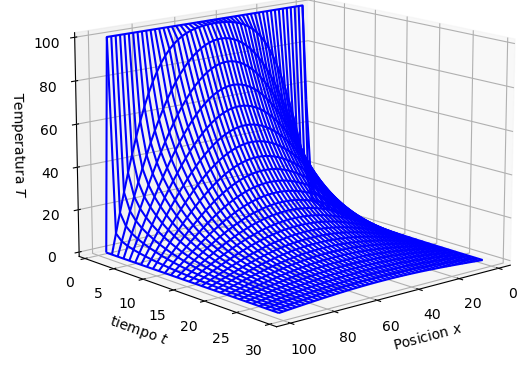
\includegraphics[width=9cm]{Img/G1.png}
			\label{}
		\end{subfigure}
		\hfill
		\begin{subfigure}[b]{0.48\textwidth}
			\centering
			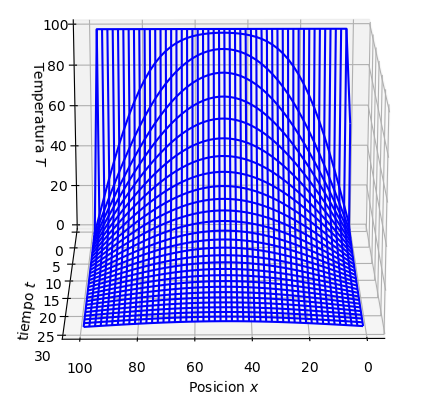
\includegraphics[width=8cm]{Img/GG.png}
			\label{}
		\end{subfigure}
		\caption{Solución numérica a la ecuación de calor para una barra de aluminio vista desde distintos ángulos.}
		\label{e}
	\end{figure}

	Recordemos nuestras condiciones de frontera:
	\begin{align}
		T(0,t) &=  0  \label{c1}\\
		T(L,t)  &= 	0  \label{c2}\\
		T(x,0) &= 100 \label{c3}
	\end{align}
	
	Analicemos los puntos en $x=0$ y $x=L$ en la figura (\ref{e}). Veamos que las líneas que conectan estos puntos siempre se mantienen en el nivel $T=0$ para cualquier $t$. Por lo tanto, las condiciones (\ref{c1}) y (\ref{c2}) se cumplen. Por otro lado, cuando $t=0$ y $x\in (0,L)$, vemos que la línea que une esos puntos se mantiene a nivel $T=100$. De esa forma la tercera condición de frontera (\ref{c3}) también se cumple.

\begin{enumerate}
	\item [\textbf{(f)}] ¿Alcanza su solución el equilibrio?¿Es estable?
\end{enumerate}
\textit{Solución.}\\
	De la figura (\ref{e}) vemos que conforme $t$ aumenta, la temperatura en la barra de aluminio disminuye. Lo cual tiene sentido, ya que en todo momento los extremos de la barra están en contacto con las barras de hielo a $T=0$. De esa forma, al transcurrir el tiempo se alcanzará el equilibrio térmico. Por lo que existirá un $t_f$ tal que $T(x,t_f) = 0$. En efecto, analizando nuestra solución vemos que para los últimos valores de $t$ en la gráfica, la temperatura en la barra es muy baja. 
	\begin{figure}[h]
		\centering
		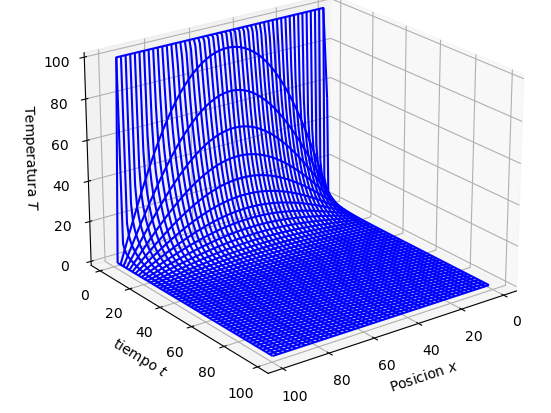
\includegraphics[width=12cm]{Img/f.png}
		\caption{Solución estable. Se aprecia que llega un punto en el eje $t$ donde se alcanza el equilibrio térmico}
		\label{}
	\end{figure}

	Así que si se proyecta más el eje $t$ como en la gráfica anterior, la barra de aluminio estará en equilibrio a $T=0$ y con ello nuestra solución es estable. 

\begin{enumerate}
	\item [\textbf{(g)}] Compare la solución numérica con la solución analítica. Conviene
	realizar una gráfica 3D de la temperatura vs posición vs tiempo e incluir las isotermas (contornos de temperatura constante).
\end{enumerate}
\textit{Solución.}\\
	Aquí utilizaremos el siguiente comando para generar las isotermas: $$\texttt{ax.plot\_surface(X, Y, Z, cmap=cm.coolwarm)}$$ 
	Por otro lado, la solución analítica está dada por:
	\begin{equation}
		T(x,t) = \sum _{n=1, 3,...}^\infty \frac{4T_0}{n\pi}\sin (k_n x) e^{\frac{-k_n^2 K}{C \rho} t} 
	\end{equation}
	Donde $k_n=\frac{n\pi}{L}$. Para nuestro problema $T_0 = 100$ y $L=1m$. Si recortamos la serie y consideramos los primeros 1000 términos obtenemos:
	\begin{equation}
		T(x,t) \approx \sum _{n=1, 3,...}^{1000} \frac{400}{n\pi}\sin (k_n x) e^{\frac{-k_n^2 K}{C \rho} t} 
	\end{equation}
	Con base en esta aproximación, graficaremos la solución analítica a partir del siguiente algoritmo que tiene como base el algoritmo creado para la solución numérica. 
	\begin{figure}[h]
		\centering
		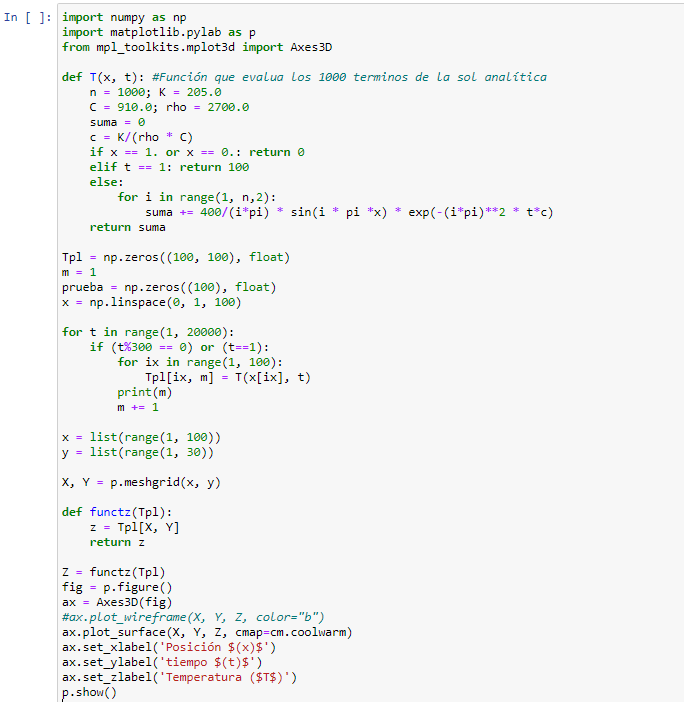
\includegraphics[width=11cm]{Img/Analitica.PNG}
		\caption{Algoritmo para graficar la solución analítica a la ecuación de Calor.}
		\label{A2}
	\end{figure}
	
	Con base en los algoritmos de las figuras (\ref{A1}) y (\ref{A2}) y la implementación del comando para generar las isotermas tenemos las siguientes gráficas para la solución numérica y analítica.

\newpage
	\begin{figure}[htp!]
		\begin{subfigure}[b]{0.48\textwidth}
			\centering
			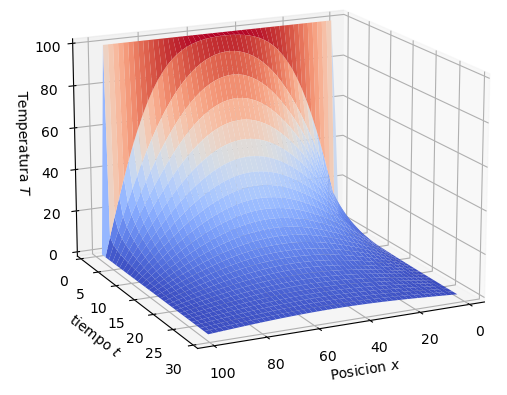
\includegraphics[width=8cm]{Img/IsotermaNumerica.png}
			\caption{Solución numérica}
			\label{}
		\end{subfigure}
		\hfill
		\begin{subfigure}[b]{0.48\textwidth}
			\centering
			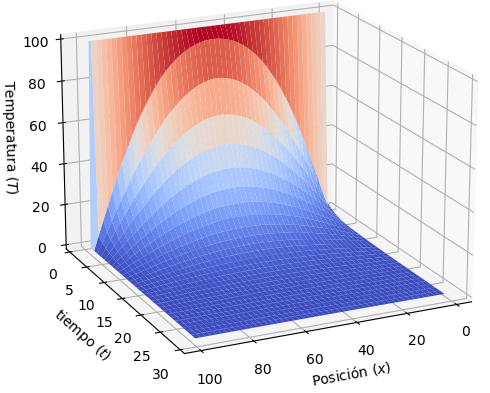
\includegraphics[width=8cm]{Img/IsotermaAnalitica.png}
			\caption{Solución analítica}
			\label{}
		\end{subfigure}
		\caption{}
		\label{}
	\end{figure}
	
	Se puede apreciar que ambas soluciones son muy parecidas entre sí. Existen pequeñas diferencias como en la curva que se genera en la parte posterior. Esta diferencia es debido a los errores que tienen los algoritmos de Forward difference y Central difference en el cálculo de la solución numérica. A pesar de ello, ambas soluciones son muy parecidas entre sí. 

\begin{enumerate}
	\item [\textbf{(h)}] ¿Qué pasa si el aluminio es sustituido por un mal conductor térmico
	como madera?
\end{enumerate}
\textit{Solución.}\\	
	Para esta parte consideraremos la madera de Pino. Para este material se tiene que:
	\begin{equation}
		K = 0.12\,\, \si{W/(m\cdot K)},\quad C = 2510\,\, \si{J/(kg\,\, K)},\quad \rho = 640 \,\,\si{kg/m^3}	\label{valoresmadera}
	\end{equation}
	Por lo que nuestra condición de estabilidad resulta:
	\begin{align*}
			\frac{\Delta t}{(\Delta x)^2} < \frac{C\rho}{2 K } \approx \num{6.69e 6}	
	\end{align*} 
	Así para $\Delta x = 0.03$ tenemos que:
	$$\Delta t < 6026$$
	Aquí tenemos mayor rango de estabilidad. El valor que se consideró fue $Delta t= 5$, obteniendo la siguiente solución donde se ha tenido que extender la cantidad de puntos a ser evaluados para apreciar mejor la solución a la ecuación de calor para el mal conductor térmico.
\newpage
	
	\begin{figure}[h]
		\centering
		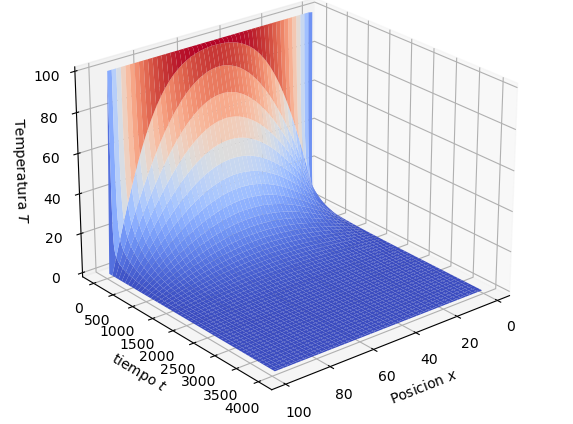
\includegraphics[width=12cm]{Img/madera.png}
		\caption{Solución estable a la ecuación de calor para madera de Pino}
		\label{}
	\end{figure}
	
	Como era de esperarse, al ser un mal conductor térmico la madera, la temperatura dentro de la barra de madera disminuye muy lentamente. Sin embargo, llegará un punto donde se alcance el equilibrio térmico. Pero para ello transcurrirá mucho tiempo.



\subsection*{\textbf{2. La vibración de una cuerda}}
	Este problema pretende estudiar las oscilaciones de una cuerda. Considere una cuerda de longitud $L$ y densidad $\rho(x)$ por unidad de longitud, atada en ambos extremos y 
	bajo una tensión $T(x)$. Suponga que el desplazamiento relativo de la cuerda respecto a su posición de equilibrio $\frac{y(x,t)}{L}$ es pequeño y que la pendiente de la cuerda $\frac{\partial y}{\partial x}$ también es pequeña.
	
\begin{enumerate}
	\item [\textbf{(a)}] Considere una sección infinitesimal de la cuerda, note que la diferencia en las componentes de las tensiones en $x$ y $x + \Delta x$ tiene por resultado una fuerza restauradora.	Demuestre que al aplicar las leyes de Newton a esta sección obtenemos la ecuación de onda:
			\begin{equation*}
				\frac{dT(x)}{dx}\frac{\partial y(x,t)}{\partial x} + T(x)\frac{\partial^2 y(x,t)}{\partial x^2} = \rho(x) \frac{\partial^2 y(x,t)}{\partial t^2}
			\end{equation*}
\end{enumerate}
\textit{Solución.}\\
	Se sabe que:
	$$\sum \vec{F}(x,y) = m \vec{a}(x,y)$$
	Proyectando en el eje $y$ tenemos:
	$$\sum F_y = m \frac{\partial^2 y(x,t)}{\partial t ^2}$$
	Notemos que para el segmento infinitesimal de cuerda tenemos que:
	$$\rho(x) = \frac{m}{\Delta x} \quad\Rightarrow\quad m = \rho (x) \Delta x$$
	Por otro lado, si consideramos las tensiones del diagrama en los puntos $x$ y $x+\Delta x$, debido a que la tensión no es constante tenemos que:
	$$\sum F_y = \left.\left( T(x') \sin \theta \right)\right|_{x' = x + \Delta x} -\left.\left( T(x') \sin \theta \right)\right|_{x' = x}$$
	El signo menos se debe a que las fuerzas van en sentidos contrarios. Luego, debido a que $\theta$ es muy pequeño y la pendiente también lo es, podemos hacer:
	$$\sin\theta \approx =\tan\theta\approx\frac{\partial y(x,t)}{\partial x}$$
	Por lo que:
	\begin{align*}
	\sum F_y &\approx \left.\left( T(x') \frac{\partial y(x',t)}{\partial x} \right)\right|_{x' = x + \Delta x} -\left.\left( T(x') \frac{\partial y(x',t)}{\partial x} \right)\right|_{x' = x}	\\
	&= T(x+\Delta x) \frac{\partial y(x+\Delta x,t)}{\partial x} - T(x)\frac{\partial y(x,t)}{\partial x}	\\
	&=  T(x+\Delta x) \frac{\partial y(x+\Delta x,t)}{\partial x} - T(x)\frac{\partial y(x,t)}{\partial x} + T(x) \frac{\partial y(x+\Delta x, t)}{\partial x} -  T(x) \frac{\partial y(x+\Delta x, t)}{\partial x}	\\
	&=\frac{\partial y(x+\Delta x, t)}{\partial x}\left[ T(x +\Delta x) - T(x)\right]+ T(x)\left[\frac{\partial y(x+\Delta x, t)}{\partial x}- \frac{\partial y(x, t)}{\partial x}\right]
	\end{align*}
	Donde hemos sumado y restado un término para poder obtener el resultado anterior. De esta forma, se sigue que:
	$$\sum F_y = m\frac{\partial^2 y(x, t)}{\partial t^2}$$
	\begin{align*}
		\Rightarrow \frac{\partial y(x+\Delta x, t)}{\partial x}\left[ T(x +\Delta x) - T(x)\right]+ T(x)\left[\frac{\partial y(x+\Delta x, t)}{\partial x}- \frac{\partial y(x, t)}{\partial x}\right] &= \rho(x) \Delta x \frac{\partial^2 y(x,t)}{\partial t^2}	\\
		\Rightarrow \frac{\partial y(x+\Delta x, t)}{\partial x}\left[ \frac{T(x +\Delta x) - T(x)}{\Delta x}\right]+ T(x)\left[\frac{\frac{\partial y(x+\Delta x, t)}{\partial x}- \frac{\partial y(x, t)}{\partial x}}{\Delta x}\right]&=  \rho(x)\frac{\partial^2 y(x,t)}{\partial t^2}
	\end{align*}
	Tomando el límite  $\Delta x \to 0$ y aplicando las definiciones de derivada total y parcial obtenemos:
	\begin{equation}
		\frac{\partial y(x,t)}{\partial x} \frac{dT(x)}{dx} + T(x)\frac{\partial^2 y(x,t)}{\partial x^2} = \rho (x) \frac{\partial^2 y(x,t)}{\partial t^2}	\label{Tvariable}
	\end{equation}
	Esta ecuación corresponde con  la \textit{\textbf{ecuación de onda para una cuerda densidad y tensión variable}}, que es lo que se pide en este inciso.

\begin{enumerate}
	\item [\textbf{(b)}] ¿Qué condiciones son necesarias para obtener la ecuación de onda estándar?
	\begin{equation}
	 \frac{\partial^2 y(x,t)}{\partial x^2} = \frac{1}{c^2} \frac{\partial^2 y(x,t)}{\partial t^2},\quad c=\sqrt{ \frac{T}{\rho}}
	\end{equation}
\end{enumerate}
\textit{Solución.}\\
	Para poder obtener la ecuación de onda estándar, basta considerar a la densidad $rho$ y la tensión $T$ constantes en la deducción del ejercicio anterior. Tomando estas consideraciones en la ecuación (\ref{Tvariable}) tenemos que:
	$$\frac{\partial y(x,t)}{\partial x} \cancelto{0}{ \frac{dT}{dx} } + T\frac{\partial^2 y(x,t)}{\partial x^2} = \rho \frac{\partial^2 y(x,t)}{\partial t^2}$$
	\begin{align*}
		 \Rightarrow T\frac{\partial^2 y(x,t)}{\partial x^2} &= \rho \frac{\partial^2 y(x,t)}{\partial t^2}	\\
		 \frac{\partial^2 y(x,t)}{\partial x^2} &= \frac{\rho}{T} \frac{\partial^2 y(x,t)}{\partial t^2}	\\
		 \frac{\partial^2 y(x,t)}{\partial x^2} &= \frac{1}{c^2} \frac{\partial^2 y(x,t)}{\partial t^2}
	\end{align*}

\begin{enumerate}
	\item [\textbf{(c)}] ¿Qué condiciones deben cumplirse para obtener una única solución
	a esta EDP de segundo orden? 
\end{enumerate}
\textit{Solución.}\\ Debido a que las derivadas parciales son de segundo orden tanto en la variable $x$ como en la variable $t$, debemos conocer 4 condiciones, pues al realizar separación de variables se obtienen dos soluciones para la variable $x$ y dos para $t$. \\
Las condiciones a conocer son las iniciales y de frontera. Por ejemplo, para las condiciones iniciales, uno puede considerar a la cuerda en reposo y después que en un punto de la cuerda se aplique una fuerza perturbativa. Por lo que en $t=0$, la velocidad será cero (al estar en reposo) y tendrá un desplazamiento inicial (ej. la mitad de la cuerda con pendiente positiva y la otra mitad con la misma pendiente desplazada pero negativa formando un triángulo). 
\begin{figure}[h]
	\centering
	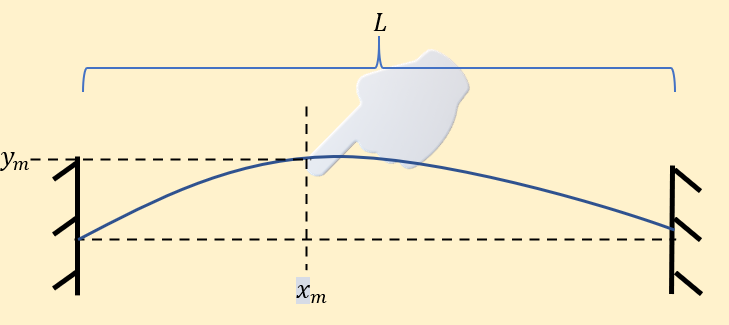
\includegraphics[width=12cm]{Img/perturba.png}
	\caption{\centering Cuerda fija en sus extremos en reposo ($t=0$) siendo jalada en un punto para generar una perturbación. Condición inicial.}
	\label{ex}
\end{figure}

	Así las condiciones iniciales considerando las ecuaciones de las rectas de la figura  (\ref{ex}) y la velocidad inicial igual a cero:
\begin{align*}
		y(x, t=0)&= \left\{\begin{array}{lcc}
								\frac{y_m}{x_m} x &   si  & 0\leq x \leq x_m \\\\
					 			\frac{y_m}{L-x_m} (L-x) &  si &  x_m<x \leq  L \\
							\end{array}\right. \\\\
		\frac{\partial y(x, t=0)}{\partial t} &=0
\end{align*}
Por otro lado,como la cuerda está sujeta de ambos extremos, las condiciones de frontera son:
\begin{align*}
	y(x=0, t) = y(x=L,t) = 0
\end{align*}

\begin{enumerate}
	\item [\textbf{(d)}] Utilice una malla de longitud $\Delta t$ en el tiempo y $\Delta x$ en el espacio para generar una solución numérica.
	$$y(x,t) = y(i\Delta x), j\Delta t)=y_ij$$
\end{enumerate}
\textit{Solución.}\\
	Al igual como se realizó en el ejercicio 1, discretizaremos nuestras variables de la siguiente forma:
	$$x = i\Delta x\quad;\quad t= j \Delta t$$
	Así es posible obtener una malla para nuestra solución numérica.
	\begin{figure}[h]
		\centering
		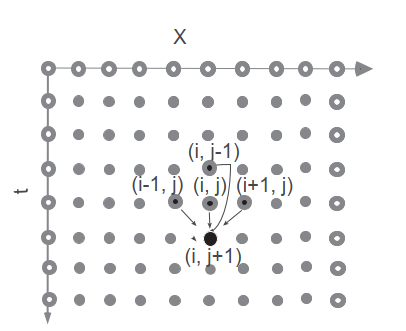
\includegraphics[width=8cm]{Img/grid.png}
		\caption{Malla discretizada}
		\label{grid}
	\end{figure}
	
	En el siguiente inciso obtendremos la ecuación de onda en diferencias.
	
\begin{enumerate}
	\item [\textbf{(e)}] Exprese las segundas derivadas de la EDP en términos de diferencias finitas, demuestre que esto resulta en la ecuación de onda en diferencias:
	$$\frac{y_{ij+1} + y_{i j-1}- 2y_{ij}}{c^2 (\Delta t)^2} = \frac{y_{i+1j} + y_{i-1 j}- 2y_{ij}}{ (\Delta x)^2}$$
\end{enumerate}
\textit{Solución.}\\	
	Retomemos la ecuación de onda:
	\begin{equation}
		\frac{\partial^2 y(x,t)}{\partial x^2} = \frac{1}{c^2} \frac{\partial^2 y(x,t)}{\partial t^2}	\label{econda}
	\end{equation}
	Usando Central difference para el cálculo de ambas derivadas obtenemos:
	\begin{align*}
		\frac{\partial^2 y}{\partial t^2} &\approx \frac{\left.\frac{\partial y}{\partial t}\right|_{t+\frac{\Delta t}{2}}  - \left.\frac{\partial y}{\partial t}\right|_{t-\frac{\Delta t}{2}}}{\Delta t}	\\
		&=\frac{\frac{y(x,t+\Delta t) - y(x,t)}{\Delta t} - \frac{y(x,t) - y(x,t-\Delta t)}{\Delta t}}{\Delta t}	\\
		&= \frac{y(x,t+\Delta t) + y(x,t-\Delta t) - 2y(x,t)}{(\Delta t)^2}	\\
		&= \frac{y_{ij+1} + y_{ij-1} -2y_{ij}}{(\Delta t )^2}
	\end{align*}
	Similarmente:
	
	\begin{align*}
		\frac{\partial^2 y}{\partial x^2} &\approx \frac{\left.\frac{\partial y}{\partial x}\right|_{x+\frac{\Delta x}{2}}  - \left.\frac{\partial y}{\partial x}\right|_{x-\frac{\Delta x}{2}}}{\Delta x}	\\
		&=\frac{\frac{y(x+\Delta x,t) - y(x,t)}{\Delta x} - \frac{y(x,t) - y(x-\Delta x,t)}{\Delta x}}{\Delta x}	\\
		&= \frac{y(x+\Delta x,t) + y(x-\Delta x,t) - 2y(x,t)}{(\Delta x)^2}	\\
		&= \frac{y_{i+1j} + y_{i-1j} -2y_{ij}}{(\Delta x )^2}
	\end{align*}
	
	Así de (\ref{econda}) claramente se obtiene lo solicitado:
	 \begin{equation}
	 	\frac{y_{i+1j} + y_{i-1 j}- 2y_{ij}}{ (\Delta x)^2} \approx \frac{y_{ij+1} + y_{i j-1}- 2y_{ij}}{c^2 (\Delta t)^2} \label{finitas}
	 \end{equation}
\begin{enumerate}
	\item [\textbf{(f)}] Demuestre que el algoritmo anterior puede reescribirse como:
	\begin{equation}\label{m3}
		y_{ij+1} = 2y_{ij} - y_{ij-1} +\frac{c^2}{c'^2}[y_{i+1j} + y_{i-1j} - 2y_{ij}]
	\end{equation}
	donde $c'= \frac{\Delta x}{\Delta t}$ es la velocidad de la malla, es decir, la razón numérica de los parámetros.
\end{enumerate}
\textit{Solución.}\\	
	Retomando el resultado del ejercicio anterior, al despejar de la ecuación (\ref{finitas}) tenemos:
	\begin{align*}
		y_{i j+1}+ y_{ij-1} -2y_{ij} &= c^2 \left(\frac{\Delta t}{\Delta x}\right)^2 [y_{i+1j} + y_{i-1 j}- 2y_{ij}]	\\
		\Rightarrow y_{i j+1}&= 2y_{ij} -y_{ij-1} + \frac{c^2}{c'^2} [y_{i+1j} + y_{i-1 j}- 2y_{ij}]
	\end{align*}

\begin{enumerate}
	\item [\textbf{(g)}] ¿Cómo entran las condiciones iniciales y las condiciones de frontera? 
\end{enumerate}
\textit{Solución.}\\	
	Retomemos las condiciones iniciales y de frontera:
	\begin{align*}
		y(x, t=0)&= \left\{\begin{array}{lcc}
			\frac{y_m}{x_m} x &   si  & 0\leq x \leq x_m \\\\
			\frac{y_m}{L-x_m} (L-x) &  si &  x_m<x \leq  L \\
		\end{array}\right. \\\\
		\frac{\partial y(x, t=0)}{\partial t} &=0 \\
		y(x=0, t) &= y(x=L,t) = 0
	\end{align*}
	Usando la notación discretizada, estas condiciones se pueden reescribir como:
	\begin{align}
		y_{1j}&= y_{Lj}=0\\
		y_{i 1}&= \left\{\begin{array}{lcc}
			\frac{y_m}{x_m} x &   si  & 1\leq i \leq m \\\\
			\frac{y_m}{L-x_m} (L-x) &  si &  m<i  \leq  L \\
		\end{array}\right. \label{m1}
	\end{align}
	Donde hemos asumido que $i=1$ corresponde a $x=0$, $i=L\to x=L$ y $j=1\to t=0$. Esta última condición permite saber la solución en todo el espacio para $t=0$.\\
	Por otro lado, la condición de la derivada usando Central difference con un salto de $\Delta t $  resulta:
	$$\frac{\partial y(x,0)}{\partial t}\approx \frac{y(x,\Delta t)- y(x,-\Delta t)}{2\Delta t}	= 0 $$
	Por lo que, si asumimos que $j=0$ corresponde a $t= -\Delta j$, $j=1$ corresponde a $t=0$ y $j=2$ a $t=\Delta t$, obtenemos que:
	$$\frac{y_{i2}- y_{i0}}{2\Delta t}	= 0 $$
	Como $\Delta t\neq 0$:
	\begin{equation}\label{m0}
		y_{i2} = y_{i0}
	\end{equation}
	Así del inciso (f), usando este resultado en la relación de recurrencia obtenemos:
	\begin{equation}\label{m2}
		y_{i2} = y_{i1} + \frac{c^2}{2c'^2} [ y_{i+1,1} + y_{i-1,1}-2y_{i1}]
	\end{equation}
	Esta ecuación usa la solución en todo el espacio para $t=0$ para propagar hacia adelante en el tiempo con un salto de $\Delta t$. \\
	
	De esta forma, al conocer la solución en todo el espacio en $t=0$ con (\ref{m1}), propagar esta solución a un tiempo posterior con (\ref{m2}) y continuar desplazando la solucióna tiempos posteriores con (\ref{m3}), es posible obtener la solución a lo largo de toda la cuerda en el tiempo que se quiera. 

\begin{enumerate}
	\item [\textbf{(h)}] La condición de Courant para la estabilidad de la solución es que:
	$$\frac{c}{c'}\leq 1$$
	¿Qué significa en términos de los pasos?
\end{enumerate}
\textit{Solución.}\\	
	Sustituyendo tenemos que:
	\begin{align*}
		\frac{c}{c'} = \frac{\frac{\sqrt{T}}{\rho}}{\frac{\Delta x}{\Delta t}}	\leq1
	\end{align*}
	Así:
	\begin{align}
		\frac{\Delta t}{\Delta x} \leq \sqrt{\frac{\rho}{T}}	\label{estabilidad2}
	\end{align}
	Esta ecuación nos dice que entre más pequeños sean los pasos en el tiempo tendremos una mejor solución, a menos que también el tiempo sea pequeño. Por lo que hay que tomar pasos en el tiempo grandes para lograr una mejor estabilidad.
	
\begin{enumerate}
	\item [\textbf{(i)}] Escriba un programa que implemente la fórmula anterior, grafique el movimiento de la cuerda, o mejor aún, produzca una animación. 
\end{enumerate}
\textit{Solución.}\\
	En esta parte optaremos por realizar un programa que genere una animación de la cuerda. Para ello se apoyará de la librería \texttt{matplolib.animation}. El algoritmo es el siguiente:
\newpage	
	\begin{figure}[h]
		\centering
		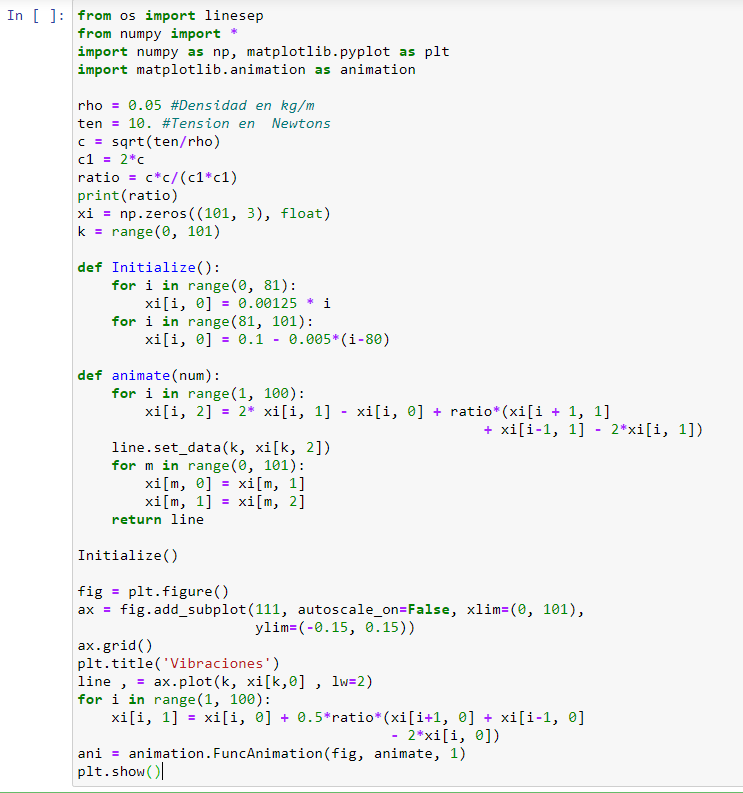
\includegraphics[width=13cm]{Img/cuerda.PNG}
		\caption{Algoritmo para generar una animación de la cuerda}
	\end{figure}
	
	La forma en como funciona el algoritmo, es que genera un arreglo de arreglos, para ir calculando los términos $y_{ij-1}$, $y_{ij}$ y $y_{ij+1}$ a partir de la realación de recurrencia (\ref{m3}). Para ello primero utiliza las otras condiciones (\ref{m1}) y (\ref{m2}). Aquí hemos considerado una cuerda de longitud 1 m, densidad  0.05 kg/m, y una tensión de 10 N. Generando así el siguiente resultado:
\newpage
	\begin{figure}[h]
		\centering
		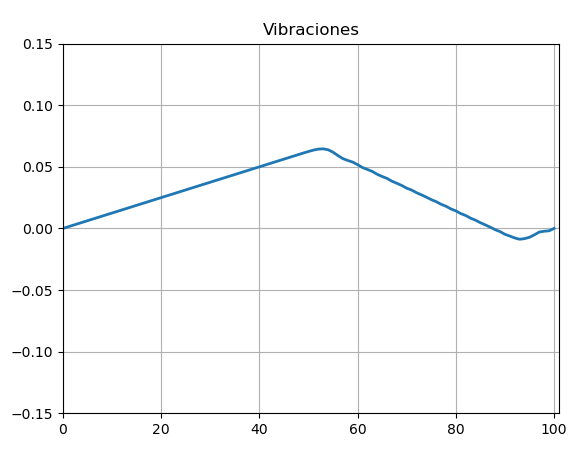
\includegraphics[width=7cm]{Img/Gcuerda.PNG}
		\caption{Comportamiento de la cuerda}
	\end{figure}
	
	Este gráfico se va moviendo con el paso del tiempo. Con forme transcurre el tiempo se desplaza la cuerda de forma que vemos las ondas generadas. En el eje $x$ se tiene la longitud de la cuerda que va de 0 a 100 cm. En el eje $y$, es la altura que va tomando la onda en la cuerda. Se puede apreciar que en los extremos de la cuerda la altura es cero, lo cual cumple con las condiciones de frontera. Además, si se deja el gráfico durante mucho tiempo, se apreciará que va disminuyendo el movimiento hasta llegar nuevamente al reposo, como era de esperarse.
	
	
	\begin{enumerate}
		\item [\textbf{(j)}] Cambie los pasos en el tiempo y el espacio en su simulación para que algunas veces satisfaga la condición de Courant y otras no.  
	\end{enumerate}
	\textit{Solución.}\\
	En nuestro algoritmo, hemos guardado la condición de Courant en la variable \texttt{ratio}. Así para tener estabilidad en nuestro programa es necesario que $\texttt{ratio}\leq 1$. Veamos como se ve nuestro resultado para distintos valores de \texttt{ratio}.
	\begin{figure}[htp!]
		\begin{subfigure}[b]{0.48\textwidth}
			\centering
			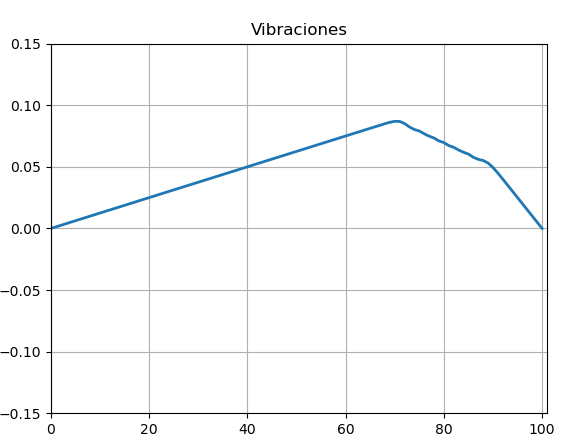
\includegraphics[width=8cm]{Img/0.1.png}
			\caption{Simulación estable para \texttt{ratio} = 0.1}
			\label{}
		\end{subfigure}
		\hfill
		\begin{subfigure}[b]{0.48\textwidth}
			\centering
			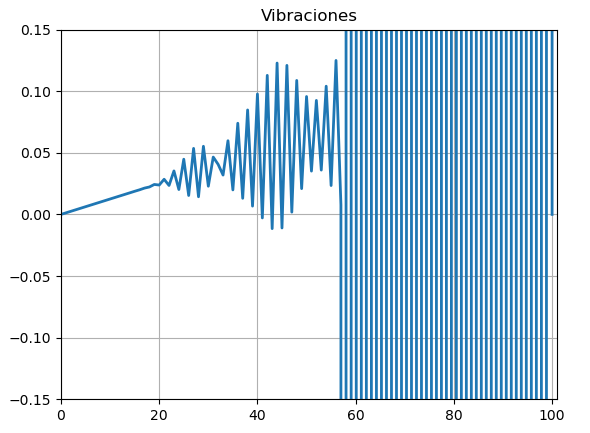
\includegraphics[width=8cm]{Img/2.png}
			\caption{Simulación inestable para \texttt{ratio} = 2.0}
			\label{}
		\end{subfigure}
		\caption{}
		\label{}
	\end{figure}

	Vemos que cuando se cumple la condición, nuestra solución es estable y se aprecia bien el comportamiento de la cuerda. Sin embargo, cuando no se cumple la condición, nuestra solución es completamente inestable. Esto se debe a que nuevamente la computadora empieza a acercarse al overflow en sus cálculos y los resultados divergen tal como se aprecia en la imagen.


\end{document}
%%%%%%%%%%%%%%%%%%%%%%%%%%%%%%%%%%%%%%%%%%%%%%%%%%%%%%%%%%%%%%%%
\begin{enumerate}
	\item [\textbf{(a)}] 
\end{enumerate}
\textit{Solución.}\\
